\documentclass[10pt, reqno]{article}		% sets document class
\usepackage[usenames,dvipsnames]{pstricks}
\usepackage{epsfig}
\usepackage{pst-grad} 				% enables gradients
\usepackage{pst-plot} 				% enables axes
\usepackage[space]{grffile} 		% enables spaces in paths
\usepackage{etoolbox} 				% enables spaces in paths
\makeatletter 						% enables spaces in paths
\patchcmd\Gread@eps{\@inputcheck#1 }{\@inputcheck"#1"\relax}{}{}
\makeatother
\usepackage[margin=1.0in]{geometry}	% sets paper size
\usepackage{amssymb}				% enables formulas
\usepackage{amsmath}				% enables formulas
\usepackage[utf8]{inputenc}			% enables diacritical input
\usepackage{graphicx}				% enables graphics
\graphicspath{ {images/} }			% sets graphics path
\usepackage{chngcntr}				% enables counter
\counterwithin{table}{subsection}	% enables table pre-labels
\counterwithin{figure}{subsection}	% enables figure pre-labels
\usepackage[labelsep=endash, labelfont=bf, font=bf]{caption}	% sets figure and caption separator
%\usepackage{indentfirst}			% enables indent on first paragraphs
\linespread{1.1}					% sets spacing to 1.5
\setlength{\parskip}{0.5em}			% sets paragraph spacing to 1m
%\usepackage{times}					% sets font to times new roman
\usepackage{wrapfig}				% enables text wrapping around figures
\usepackage{gensymb}				% enables symbols
\usepackage{endnotes}				% enables endnotes
\usepackage{afterpage}				% enables afterpage capability
\setcounter{secnumdepth}{3}			% sets counter recognitions to sssection for label capability
\numberwithin{equation}{section}
\makeatletter						% set figure labels to center
\g@addto@macro\@floatboxreset\centering
\makeatother
\usepackage{setspace}				% enables environments for spacing
\usepackage{graphicx}				% allows table usage
\usepackage{hyperref}				% enables hyperlinks
\hypersetup{colorlinks=false, linkcolor=cyan, urlcolor=cyan, linktoc=page} % sets hyperlink colors
\usepackage{accents}				% enables accents
\usepackage{textcomp} 				% enables copyright
\usepackage{tabto}					% enables tabbing
\setlength\parindent{0pt}			% sets no indents
\usepackage[framed]{mcode} 			% enables code boxes
\usepackage{titlesec}				% enables title formatting
\titleformat{\part}{\filcenter\huge\bfseries}{}{}{}
\usepackage{float}

\begin{document}

\newcommand{\stoptocwriting}{%
	\addtocontents{toc}{\protect\setcounter{tocdepth}{-5}}}
\newcommand{\resumetocwriting}{%
	\addtocontents{toc}{\protect\setcounter{tocdepth}{\arabic{tocdepth}}}}

\stoptocwriting
\part*{\underline{AERO 430 -- Numerical Simulation} \\ \Large Second-Order Linear Ordinary Differential Equation Boundary-Value Problem \\ \large Ross B. Alexander}
\resumetocwriting

\vfill

\begin{figure}[h]
	\begin{center}
	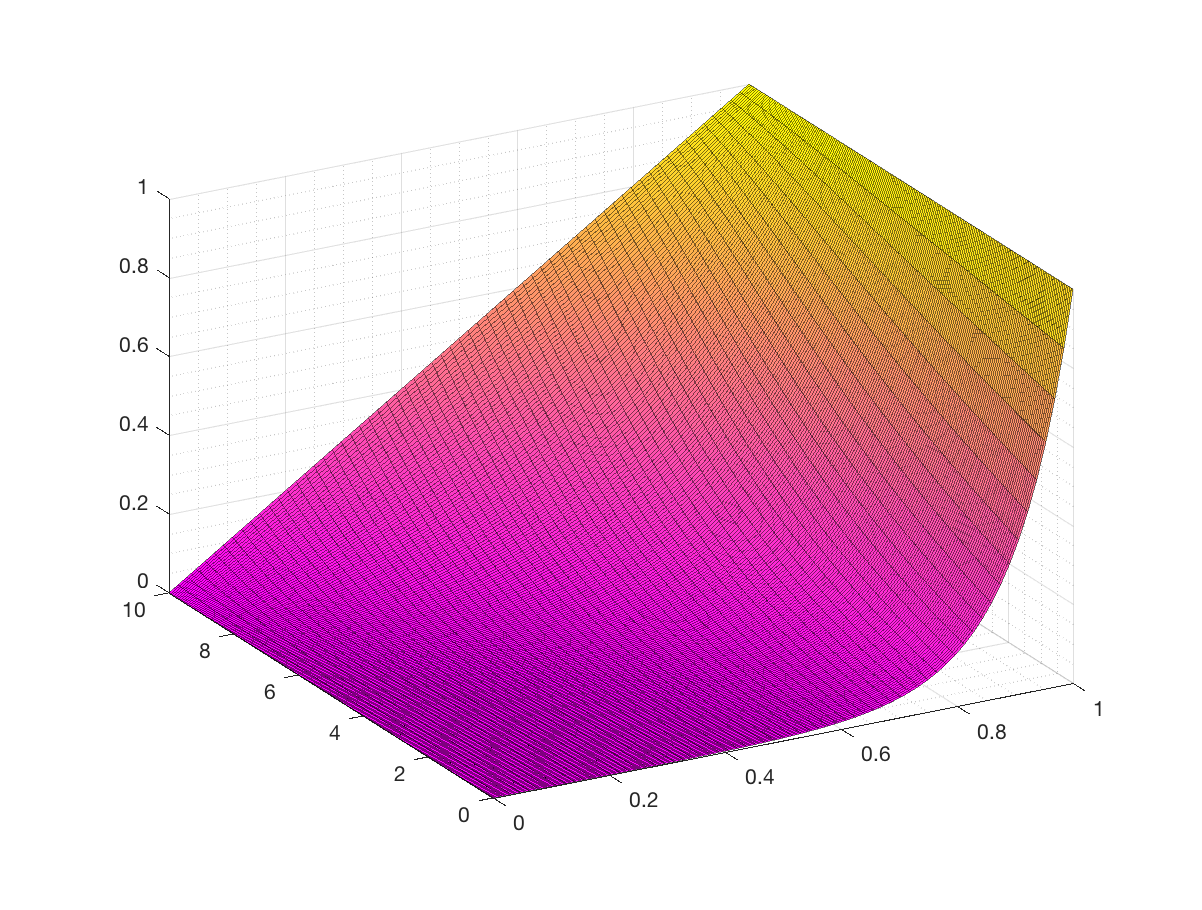
\includegraphics[width = 0.98\linewidth]{title_image}
	\end{center}
\end{figure}

\vspace{80pt}

\newpage

\tableofcontents

\newpage

\section{Model Problem}

The model second-order linear ordinary differential equation boundary-value problem consists of:
\begin{itemize}
	\item the second-order linear ordinary differential equation:
	\begin{equation}
	\pm u''(x)+k^2u(x)=k^2x \qquad x \in (0, 1)
	\end{equation}
	\item the boundary conditions:
	\begin{equation}
	u(0) = 0 \quad \textnormal{and} \quad u(1) = 0 
	\end{equation}
\end{itemize}
The model second-order linear ordinary differential equation is given with a plus-or-minus sign, as the results of the solution of each second-order linear ordinary differential equation are similar. The physical model of the positive case is that of the amplitude of standing waves for uniaxial forced vibration of a bar. The physical model for the negative case is that of (1) the temperature of a bar for uniaxial heat conduction, and (2) the deflection of a beam for uniaxial deformation with distributed elastic restraint.

\vfill

\begin{figure}[H]
	\begin{center}
		\includegraphics[width = 0.7\linewidth]{model_problem_image}
	\end{center}
\end{figure}

\vspace{50pt}

\newpage

\section{Analytical Solution}

\subsection{Positive ODE}

The following equation is the positive second-order linear ordinary differential equation (ODE).
\begin{equation}
u''(x)+k^2u(x)=k^2x
\end{equation}

\subsubsection{Homogeneous Solution}

Let the homogeneous solution to the positive ODE be defined as $u_h(x)$. Then, $u_h(x)$ must satisfy the following homogeneous ODE.
\begin{equation}
u''_h(x) + k^2u_h(x) = 0
\end{equation}
The solution of the homogeneous ODE is assumed to be of the form: 
\begin{equation}
u_h(x) = e^{\lambda x}
\end{equation}
Taking the second-derivative of $u_h(x)$, substituting the second-derivative into the homogeneous ODE, and reducing the equation yields the \textbf{characteristic equation}.
\begin{equation}
u''_h(x) = \lambda^2 e^{\lambda x}
\end{equation}
\begin{equation}
\lambda^2 e^{\lambda x} + k^2e^{\lambda x} = 0
\end{equation}
\begin{equation}
\mathbf{\lambda^2 + k^2 = 0}
\end{equation}
Solving for $\lambda$ yields:
\begin{equation}
\lambda = \pm ik
\end{equation}
The homogenous solution $u_h(x)$ is then:
\begin{equation}
u_h(x) = \alpha e^{ikx} + \beta e^{-ikx}
\end{equation}
Making a transformation with the following relations, a more sophistocated solution can be developed:
\begin{equation}
\gamma = \frac{\alpha+\beta}{2} \quad \textnormal{and} \quad \delta = i\frac{\alpha-\beta}{2}
\end{equation}
\begin{equation}
u_h(x) = \gamma \frac{e^{ikx}+e^{-ikx}}{2} + \delta \frac{e^{ikx}-e^{-ikx}}{2i}
\end{equation}
\begin{equation}
\mathbf{u_h(x) = \gamma cos(kx) + \delta sin(kx)}
\end{equation}

\subsubsection{Particular Solution}

Let the particular solution to the positive ODE be defined as $u_p(x)$. Then, $u_p(x)$ must satisfy the ODE:
\begin{equation}
u''_p(x) + k^2u_p(x) = k^2x
\end{equation}
The second-derivative of $u_p(x)$, $u''_p(x)$, is assumed to be zero, and thus yields the particular solution $u_p(x)$:
\begin{equation}
k^2u_p(x) = k^2x
\end{equation}
\begin{equation}
\mathbf{u_p(x) = x}
\end{equation}

\subsubsection{Boundary Conditions}

Given that $u_h(x)$ is a solution to the homogeneous ODE and $u_p(x)$ is a solution to the ODE, then the combination of $u_h(x)$ and $u_p(x)$ is also a solution to the ODE.
\begin{equation}
u(x) = u_h(x) + u_p(x)
\end{equation}
\begin{equation}
u(x) = \gamma cos(kx) + \delta sin(kx) + x
\end{equation}
The boundary conditions for the model problem are:
\begin{equation}
u(0) = 0 \quad \textnormal{and} \quad u(1) = 0 
\end{equation}
Applying the first boundary condition, $u(0) = 0$, we get that $\gamma = 0$:
\begin{equation}
u(0) = 0 = \gamma cos(0) + \delta sin(0) + 0
\end{equation}
\begin{equation}
\gamma = 0
\end{equation}
Applying the second boundary condition, $u(1) = 0$, we get that $\delta = \frac{-1}{sin(k)}$:
\begin{equation}
u(1) = 0 = \delta sin(k) + 1
\end{equation}
\begin{equation}
\delta = \frac{-1}{sin(k)}
\end{equation}

\subsubsection{Analytical Solution}

Thus, it is shown that for the positive second-order linear ordinary differential equation with specified boundary conditions (reproduced below) that $u(x)$ is a solution to the differential equation on $x \in (0, 1)$.
\begin{equation}
u''(x)+k^2u(x)=k^2x \qquad x \in (0, 1)
\end{equation}
\begin{equation}
u(0) = 0 \quad \textnormal{and} \quad u(1) = 0 
\end{equation}
\begin{equation}
\mathbf{u(x) = x - \frac{sin(kx)}{sin(k)}}
\end{equation}

\subsection{Negative ODE}

The following equation is the negative second-order linear ordinary differential equation (ODE).
\begin{equation}
-u''(x)+k^2u(x)=k^2x
\end{equation}

\subsubsection{Homogeneous Solution}

Let the homogeneous solution to the negative ODE be defined as $u_h(x)$. Then, $u_h(x)$ must satisfy the following homogeneous ODE.
\begin{equation}
-u''_h(x) + k^2u_h(x) = 0
\end{equation}
The solution of the homogeneous ODE is assumed to be of the form: 
\begin{equation}
u_h(x) = e^{\lambda x}
\end{equation}
Taking the second-derivative of $u_h(x)$, substituting the second-derivative into the homogeneous ODE, and reducing the equation yields the \textbf{characteristic equation}.
\begin{equation}
u''_h = \lambda^2 e^{\lambda x}
\end{equation}
\begin{equation}
-\lambda^2 e^{\lambda x} + k^2e^{\lambda x} = 0
\end{equation}
\begin{equation}
\mathbf{-\lambda^2 + k^2 = 0}
\end{equation}
Solving for $\lambda$ yields:
\begin{equation}
\lambda = \pm k
\end{equation}
The homogenous solution $u_h(x)$ is then:
\begin{equation}
u_h(x) = \alpha e^{kx} + \beta e^{-kx}
\end{equation}
By making a transformation with the following relations, a more sophistocated solution can be developed:
\begin{equation}
\gamma = \frac{\alpha+\beta}{2} \quad \textnormal{and} \quad \delta = \frac{\alpha-\beta}{2}
\end{equation}
\begin{equation}
u_h(x) = \gamma \frac{e^{kx}+e^{-kx}}{2} + \delta \frac{e^{kx}-e^{-kx}}{2}
\end{equation}
\begin{equation}
\mathbf{u_h(x) = \gamma cosh(kx) + \delta sinh(kx)}
\end{equation}

\subsubsection{Particular Solution}

Let the particular solution to the negative ODE be defined as $u_p(x)$. Then, $u_p(x)$ must satisfy the ODE:
\begin{equation}
-u''_p(x) + k^2u_p(x) = k^2x
\end{equation}
The second-derivative of $u_p(x)$, $u''_p(x)$, is assumed to be zero, and thus yields the particular solution $u_p(x)$:
\begin{equation}
k^2u_p(x) = k^2x
\end{equation}
\begin{equation}
\mathbf{u_p(x) = x}
\end{equation}

\subsubsection{Boundary Conditions}

Given that $u_h(x)$ is a solution to the homogeneous ODE and $u_p(x)$ is a solution to the ODE, then the combination of $u_h(x)$ and $u_p(x)$ is also a solution to the ODE.
\begin{equation}
u(x) = u_h(x) + u_p(x)
\end{equation}
\begin{equation}
u(x) = \gamma cosh(kx) + \delta sinh(kx) + x
\end{equation}
The boundary conditions for the model problem are:
\begin{equation}
u(0) = 0 \quad \textnormal{and} \quad u(1) = 0 
\end{equation}
Applying the first boundary condition, $u(0) = 0$, we get that $\gamma = 0$:
\begin{equation}
u(0) = 0 = \gamma cosh(0) + \delta sinh(0) + 0
\end{equation}
\begin{equation}
\gamma = 0
\end{equation}
Applying the second boundary condition, $u(1) = 0$, we get that $\delta = \frac{-1}{sinh(k)}$:
\begin{equation}
u(1) = 0 = \delta sinh(k) + 1
\end{equation}
\begin{equation}
\delta = \frac{-1}{sinh(k)}
\end{equation}

\subsubsection{Analytical Solution}

Thus, it is shown that for the negative second-order linear ordinary differential equation with specified boundary conditions (reproduced below) that $u(x)$ is a solution to the differential equation on $x \in (0, 1)$.
\begin{equation}
-u''(x)+k^2u(x)=k^2x \qquad x \in (0, 1)
\end{equation}
\begin{equation}
u(0) = 0 \quad \textnormal{and} \quad u(1) = 0 
\end{equation}
\begin{equation}
\mathbf{u(x) = x - \frac{sinh(kx)}{sinh(k)}}
\end{equation}

\newpage

\section{Numerical Methods}

\subsection{Second-Order Second-Derivative Finite Difference Method}

\subsubsection{Derivation}

Developing the Taylor series for $u(x)$ in the vicinity of $x = i$:
\begin{equation}
u_{i-1} = u_i - \Delta x u'_i + \frac{\Delta x^2}{2} u''_i - \frac{\Delta x^3}{6} u^{(3)}_i + \frac{\Delta x^4}{24} u^{(4)}_i + \mathcal{O}(\Delta x^5)
\end{equation}
\begin{equation}
u_{i+1} = u_i + \Delta x u'_i + \frac{\Delta x^2}{2} u''_i + \frac{\Delta x^3}{6} u^{(3)}_i + \frac{\Delta x^4}{24} u^{(4)}_i + \mathcal{O}(\Delta x^5)
\end{equation}
Adding the Taylor series for $u_{i-1}$ and $u_{i+1}$ and canceling terms:
\begin{equation}
u_{i+1} + u_{i-1} = 2u_i + \Delta x^2 u''_i + \mathcal{O}(\Delta x^4)
\end{equation}
Rearranging terms to solve for $u''_i$:
\begin{equation}
u''_i = \frac{u_{i+1} - 2u_i + u_{i-1}}{\Delta x^2} + \mathcal{O}(\Delta x^2) 
\end{equation}

From this specific second-derivative formulation using the finite difference method, the approximation can be observed to be second-order ($\mathcal{O}(\Delta x^2)$).

\subsubsection{Results -- Positive ODE}

\begin{figure}[H]
	\begin{center}
		\includegraphics[height = 0.55\linewidth]{positive_ode_order_2_k_1}
		\caption{Positive ODE -- 2nd-Order FDM for $k = 1$}
	\end{center}
\end{figure}

\begin{figure}[H]
	\begin{center}
		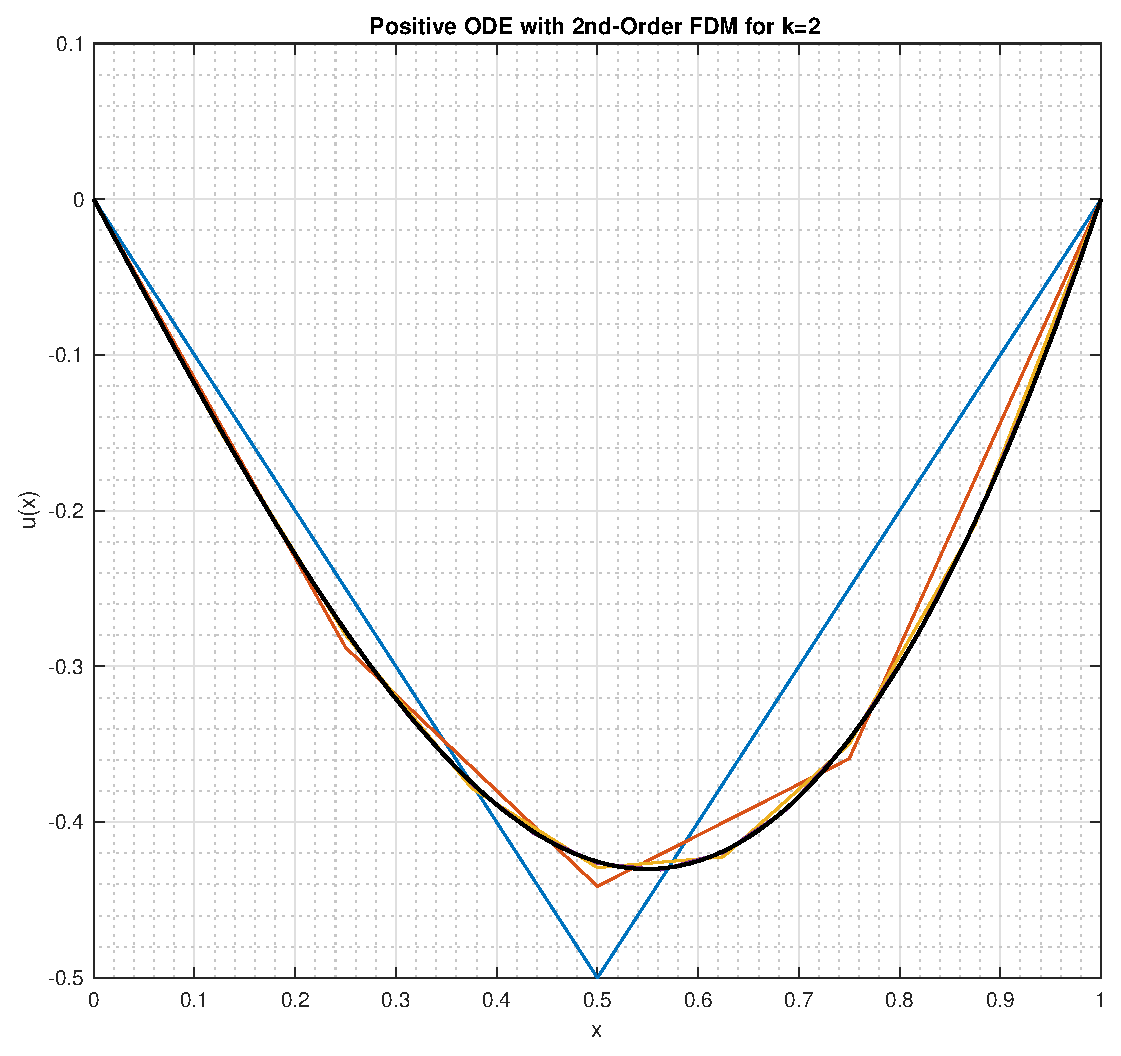
\includegraphics[height = 0.55\linewidth]{positive_ode_order_2_k_2}
		\caption{Positive ODE -- 2nd-Order FDM for $k = 2$}
	\end{center}
\end{figure}

\vfill

\begin{figure}[H]
	\begin{center}
		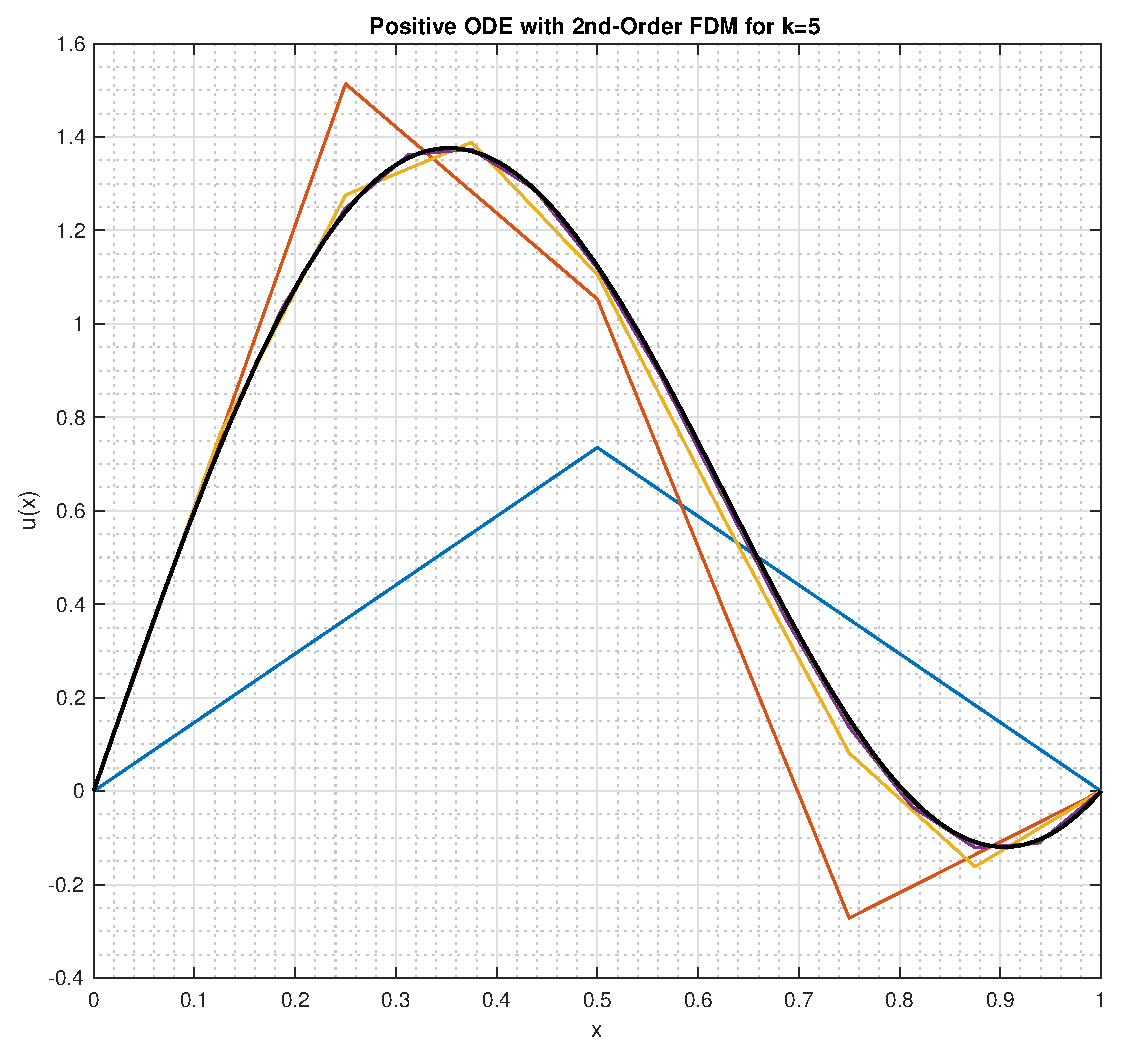
\includegraphics[height = 0.55\linewidth]{positive_ode_order_2_k_5}
		\caption{Positive ODE -- 2nd-Order FDM for $k = 5$}
	\end{center}
\end{figure}

\begin{figure}[H]
	\begin{center}
		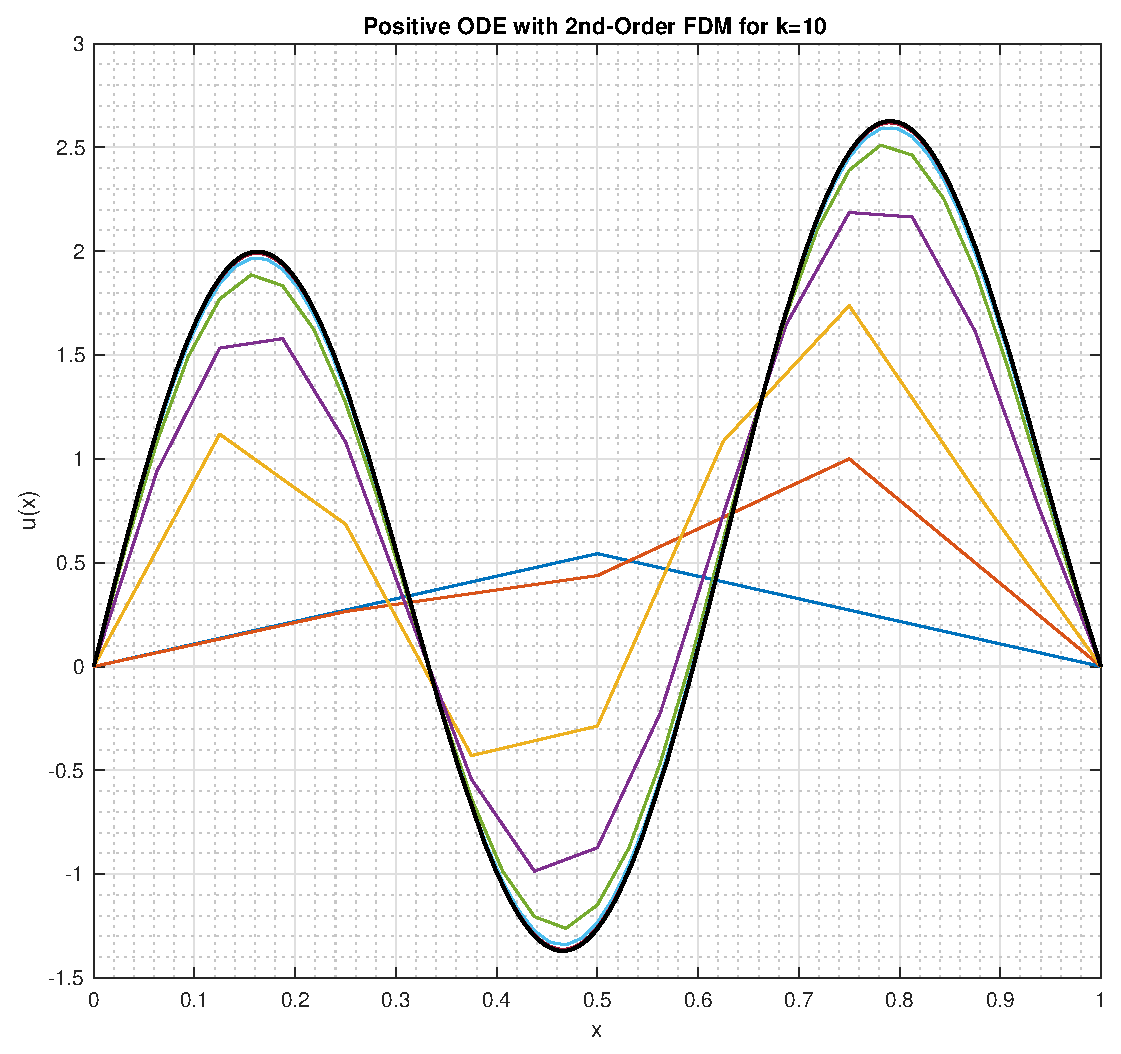
\includegraphics[height = 0.55\linewidth]{positive_ode_order_2_k_10}
		\caption{Positive ODE -- 2nd-Order FDM for $k = 10$}
	\end{center}
\end{figure}

\vfill

\begin{figure}[H]
	\begin{center}
		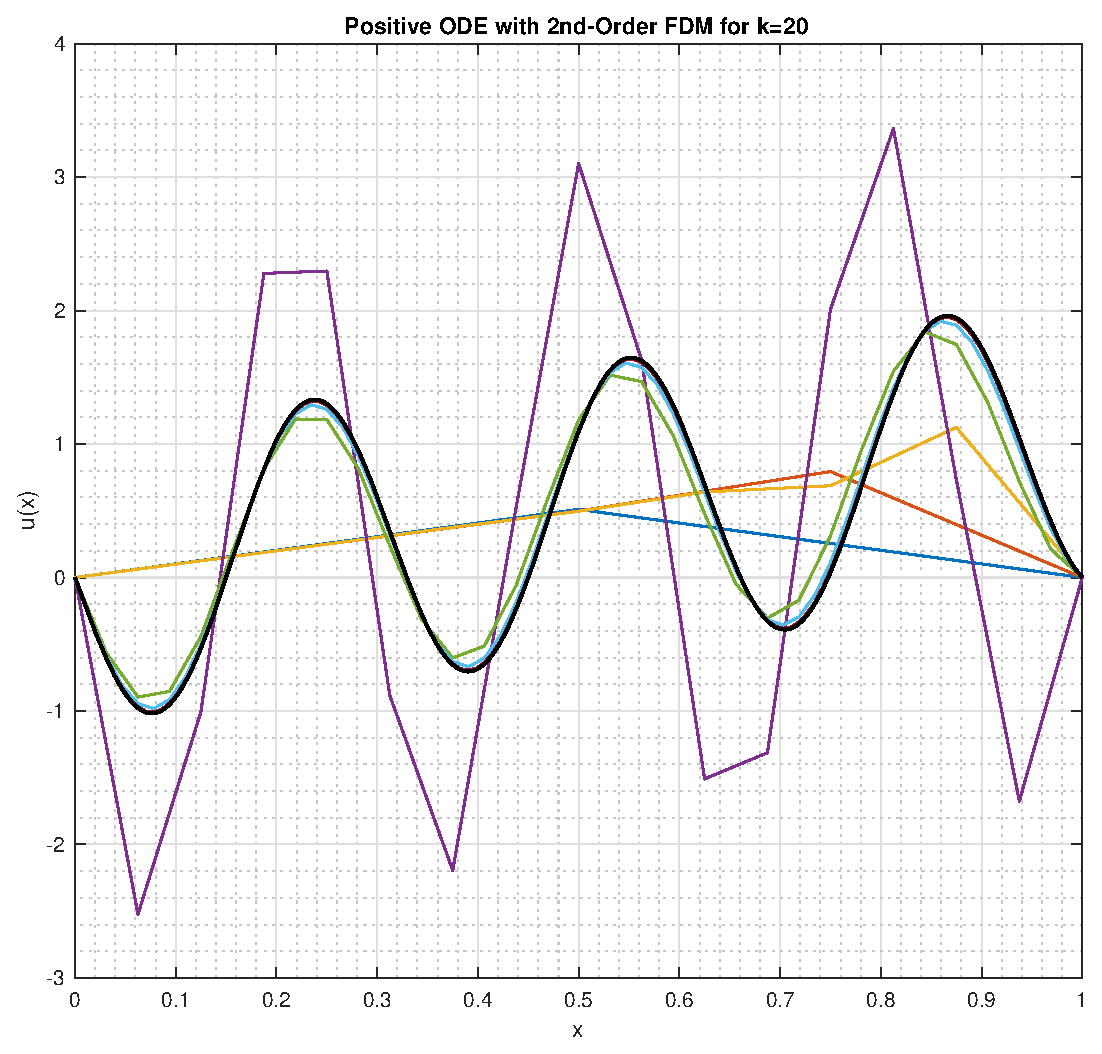
\includegraphics[height = 0.55\linewidth]{positive_ode_order_2_k_20}
		\caption{Positive ODE -- 2nd-Order FDM for $k = 20$}
	\end{center}
\end{figure}

\subsubsection{Discussion -- Positive ODE}

For the positive ODE, the analytical solution oscillates and generally increases in the amplitude of the oscillations as $k$ increases. Like expected, as mesh size is decreased, the approximation of the solution to the model problem approaches the analytical solution. At high values of $k$ ($k \ge 20$), the mesh size $\Delta x = (1/2)^6$ begins to be insufficient to resolve the solution as the number of complete cycles on the domain increases. This insufficiency appears to propagate for higher values of $k$ as overall resolution is poorer for all mesh sizes. It is likely that a fourth-order approximation of the second-derivative term would yield better agreement with the analytical solution.

\subsubsection{Results -- Negative ODE}

\begin{figure}[H]
	\begin{center}
		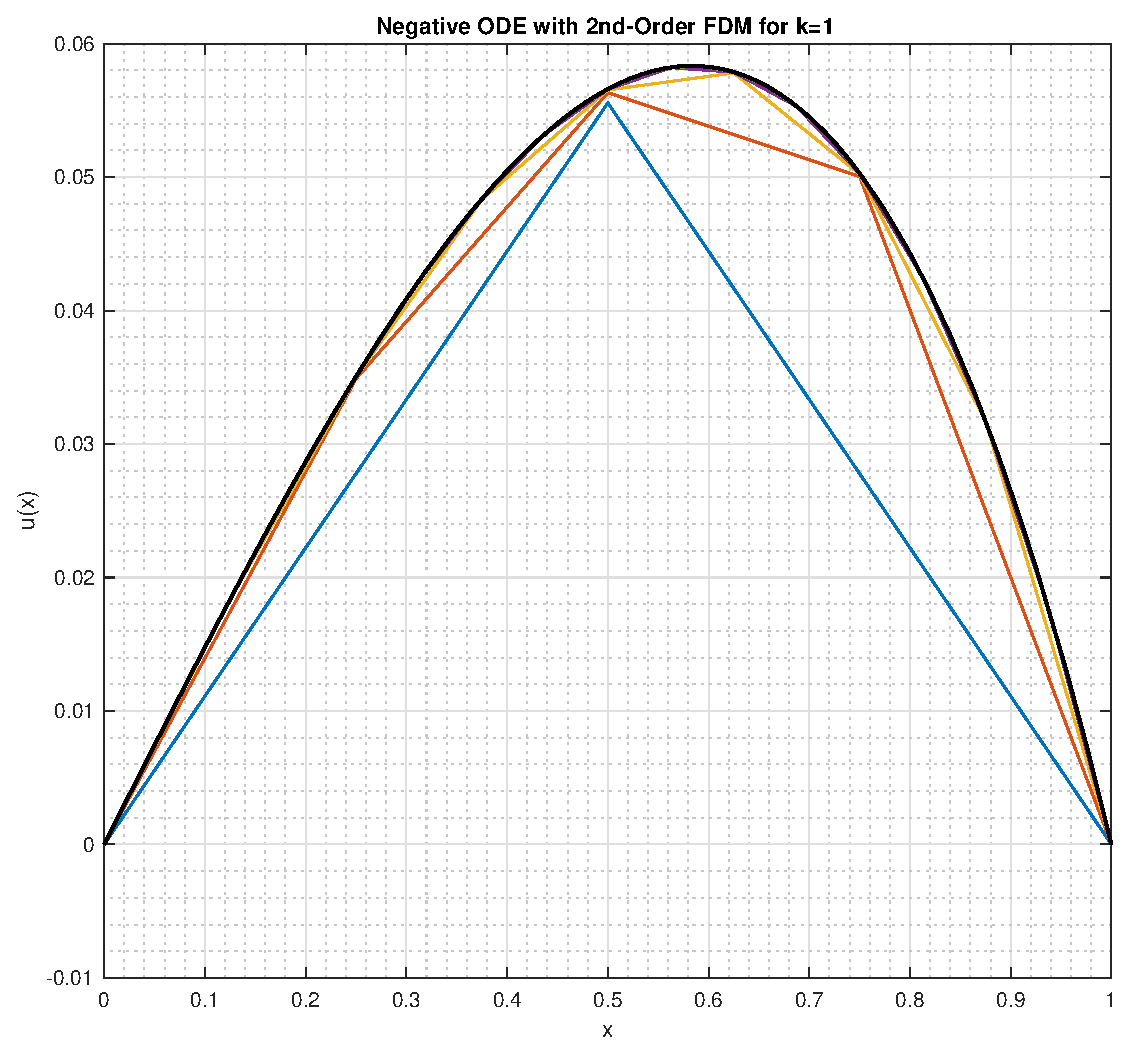
\includegraphics[height = 0.55\linewidth]{negative_ode_order_2_k_1}
		\caption{Negative ODE -- 2nd-Order FDM for $k = 1$}
	\end{center}
\end{figure}

\begin{figure}[H]
	\begin{center}
		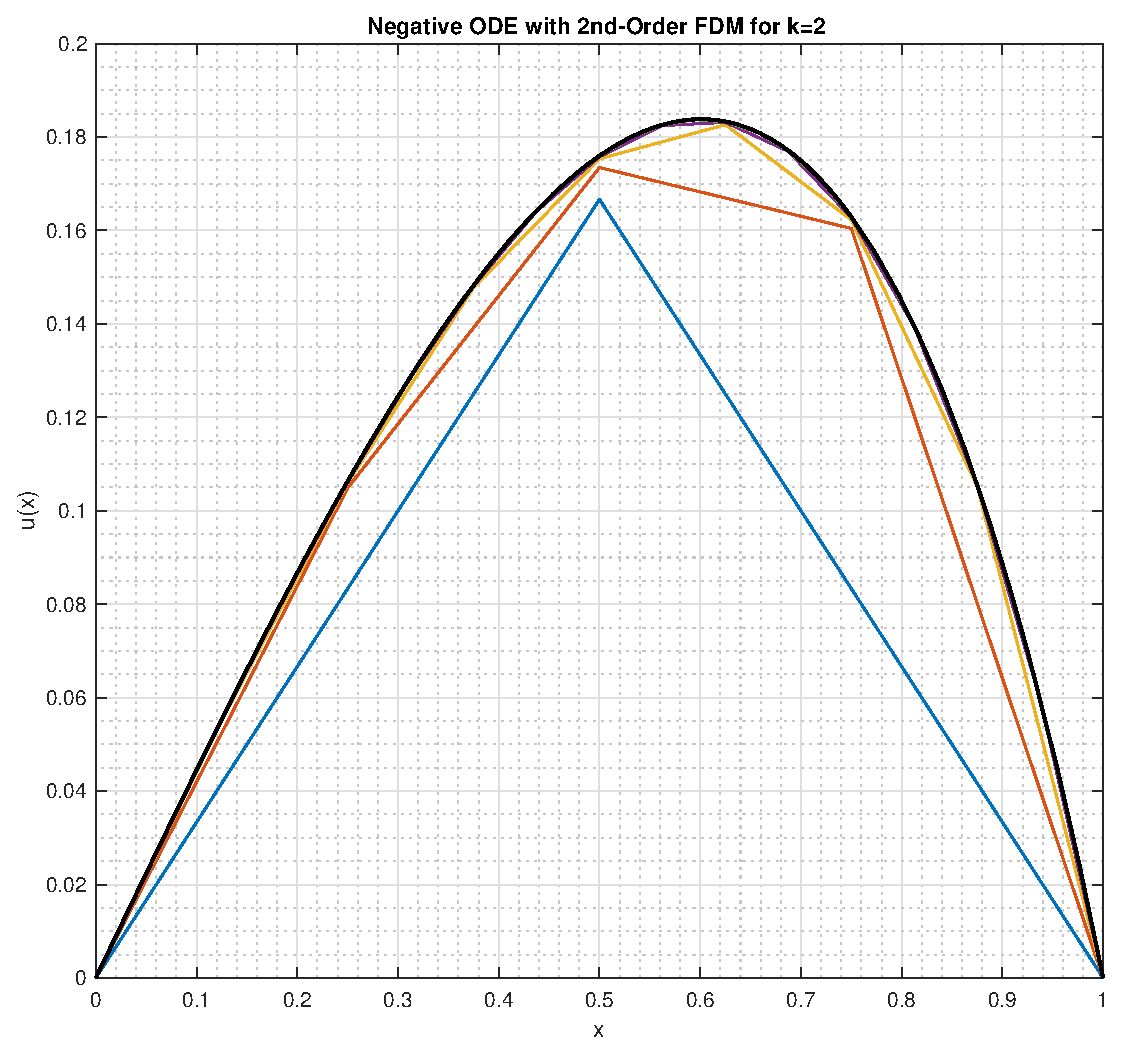
\includegraphics[height = 0.55\linewidth]{negative_ode_order_2_k_2}
		\caption{Negative ODE -- 2nd-Order FDM for $k = 2$}
	\end{center}
\end{figure}

\vfill

\begin{figure}[H]
	\begin{center}
		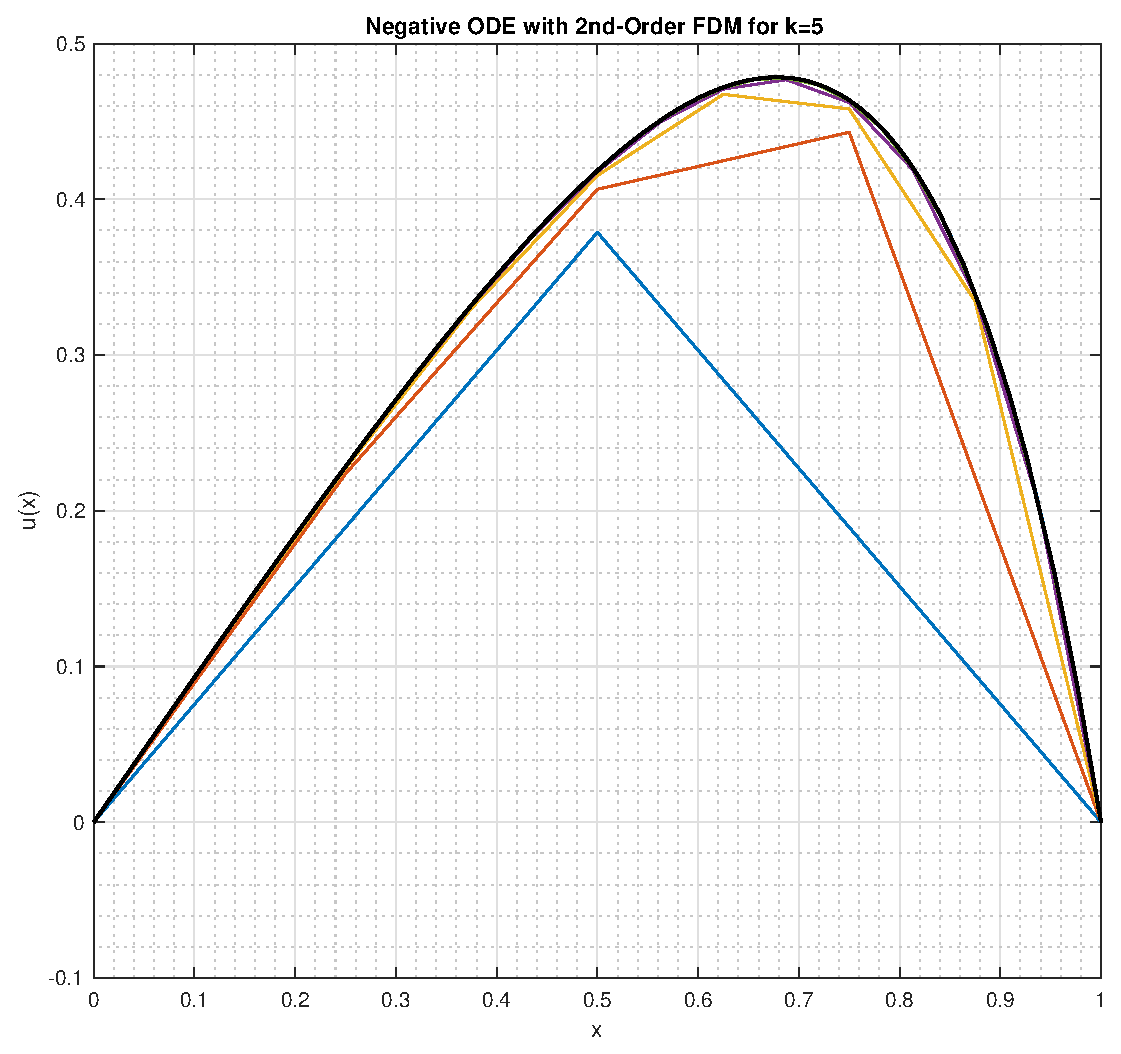
\includegraphics[height = 0.55\linewidth]{negative_ode_order_2_k_5}
		\caption{Negative ODE -- 2nd-Order FDM for $k = 5$}
	\end{center}
\end{figure}

\begin{figure}[H]
	\begin{center}
		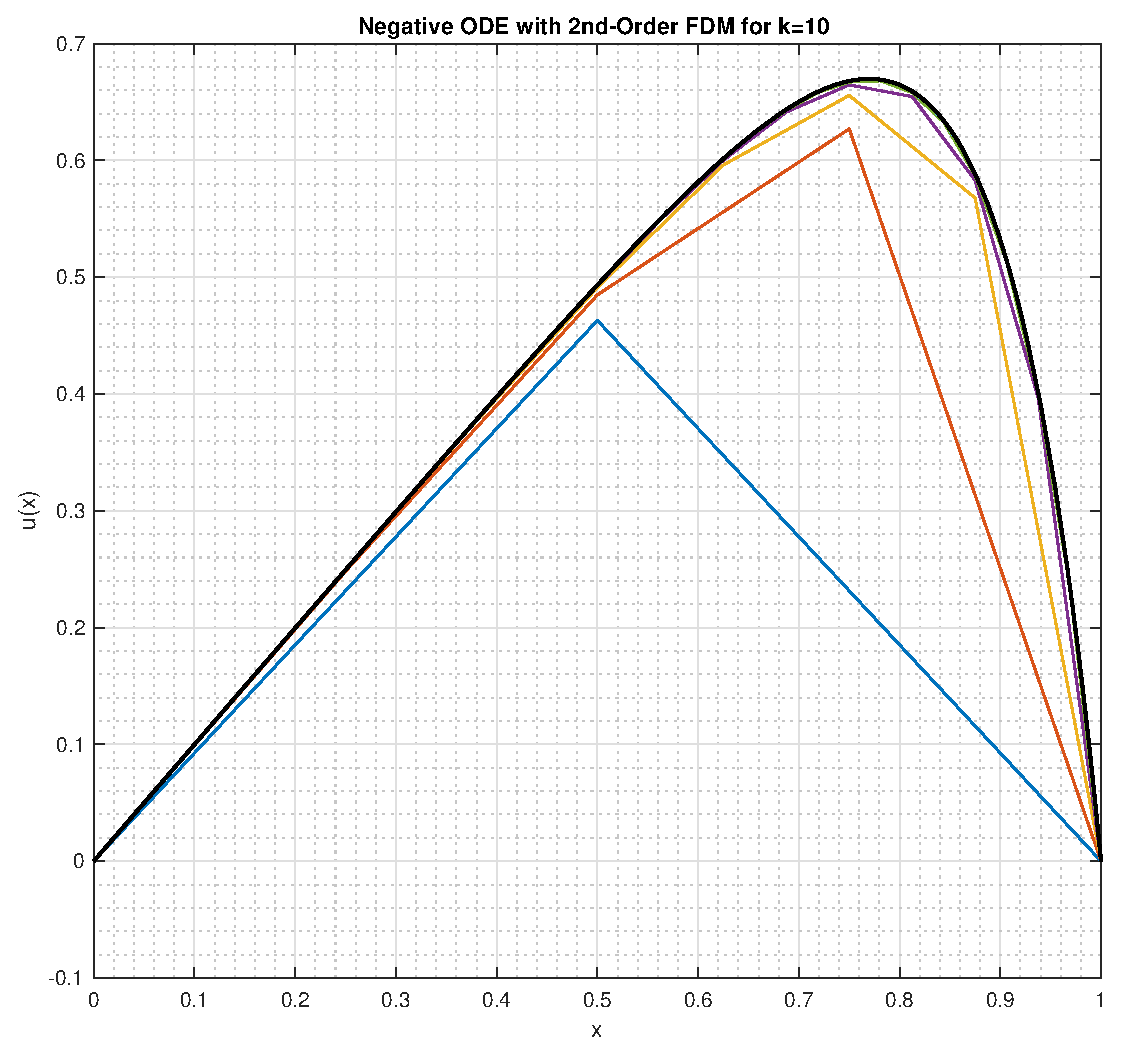
\includegraphics[height = 0.55\linewidth]{negative_ode_order_2_k_10}
		\caption{Negative ODE -- 2nd-Order FDM for $k = 10$}
	\end{center}
\end{figure}

\vfill

\begin{figure}[H]
	\begin{center}
		\includegraphics[height = 0.55\linewidth]{negative_ode_order_2_k_20}
		\caption{Negative ODE -- 2nd-Order FDM for $k = 20$}
	\end{center}
\end{figure}

\subsubsection{Discussion -- Negative ODE}

For the negative ODE, the analytical solution asymptotically approaches the line $y = x$ as $k$ increases. Like expected, as mesh size is decreased, the approximation of the solution to the model problem approaches the analytical solution. Unlike the positive ODE, at high values of $k$ ($k \ge 20$), the mesh size $\Delta x = (1/2)^6$ is sufficient to resolve the solution as difference between different values of $k$ is increasingly negligible. It is likely that a fourth-order approximation of the second-derivative term would yield better agreement with and quicker convergence to the analytical solution.

%\subsection{Fourth-Order Second-Derivative Finite Difference Method}
%
%\subsubsection{Derivation}
%
%\subsubsection{Results -- Positive ODE}
%
%\begin{figure}[H]
%	\begin{center}
%		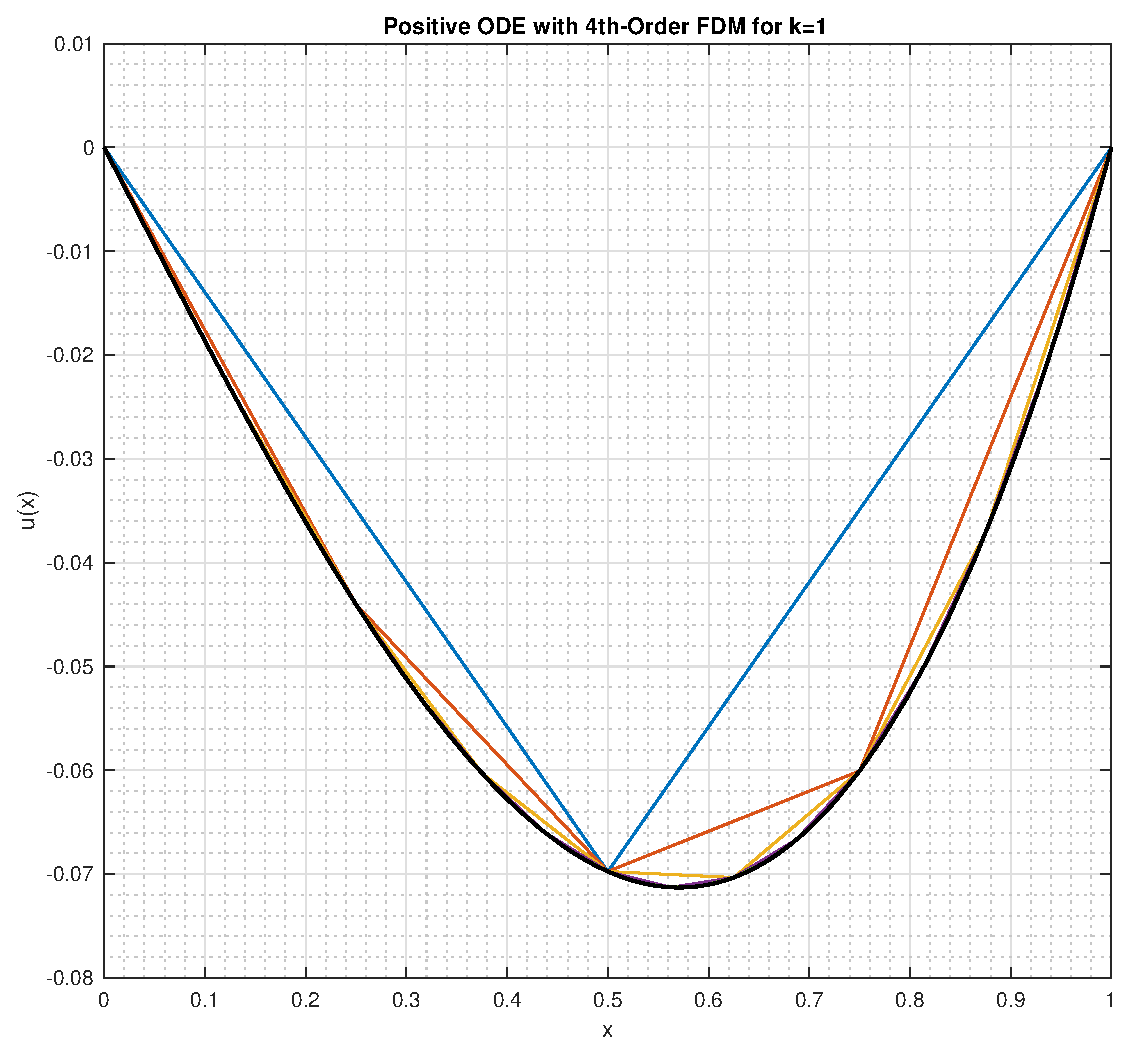
\includegraphics[height = 0.55\linewidth]{positive_ode_order_4_k_1}
%		\caption{Positive ODE -- 4th-Order FDM for $k = 1$}
%	\end{center}
%\end{figure}
%
%\begin{figure}[H]
%	\begin{center}
%		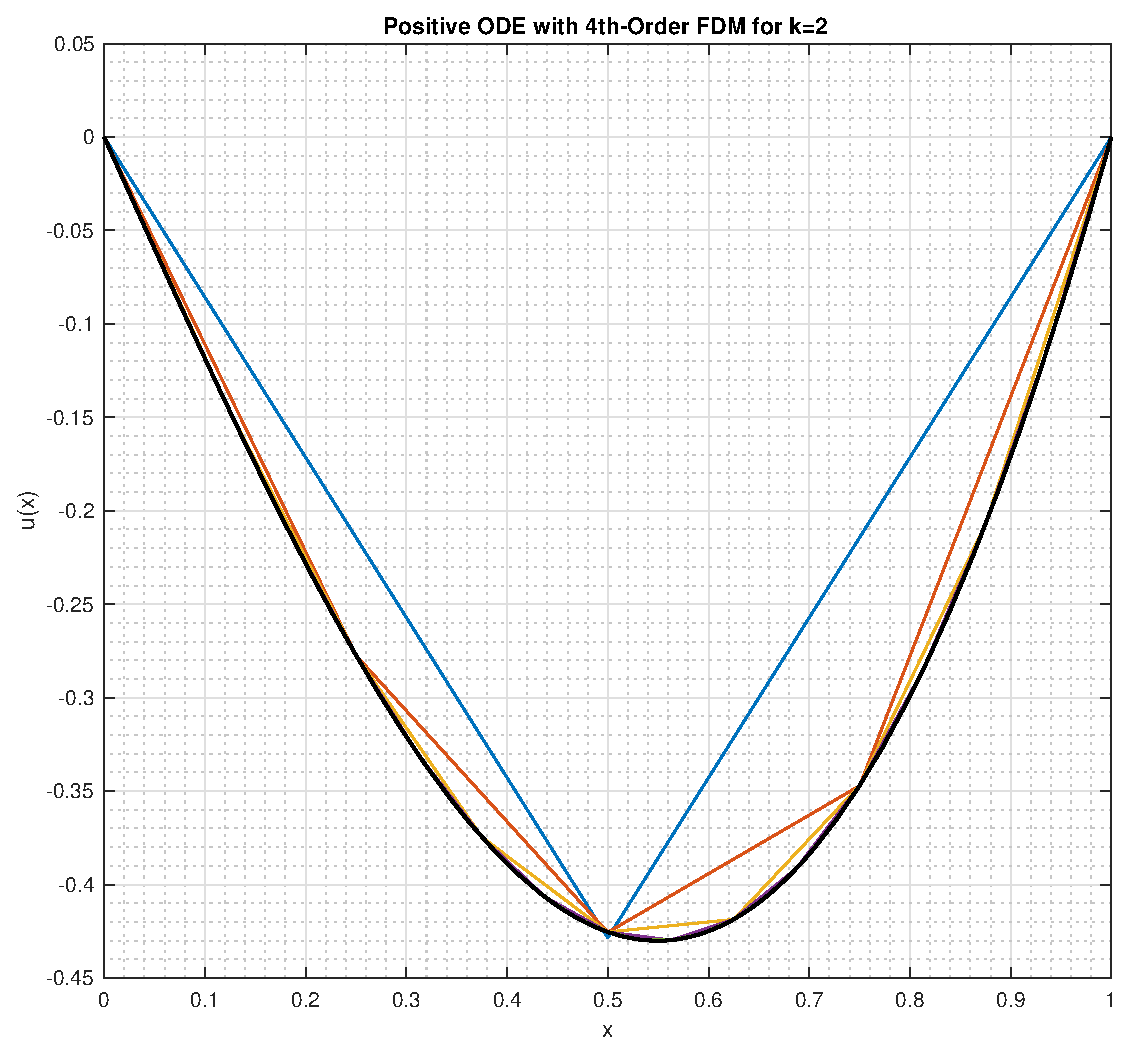
\includegraphics[height = 0.55\linewidth]{positive_ode_order_4_k_2}
%		\caption{Positive ODE -- 4th-Order FDM for $k = 2$}
%	\end{center}
%\end{figure}
%
%\begin{figure}[H]
%	\begin{center}
%		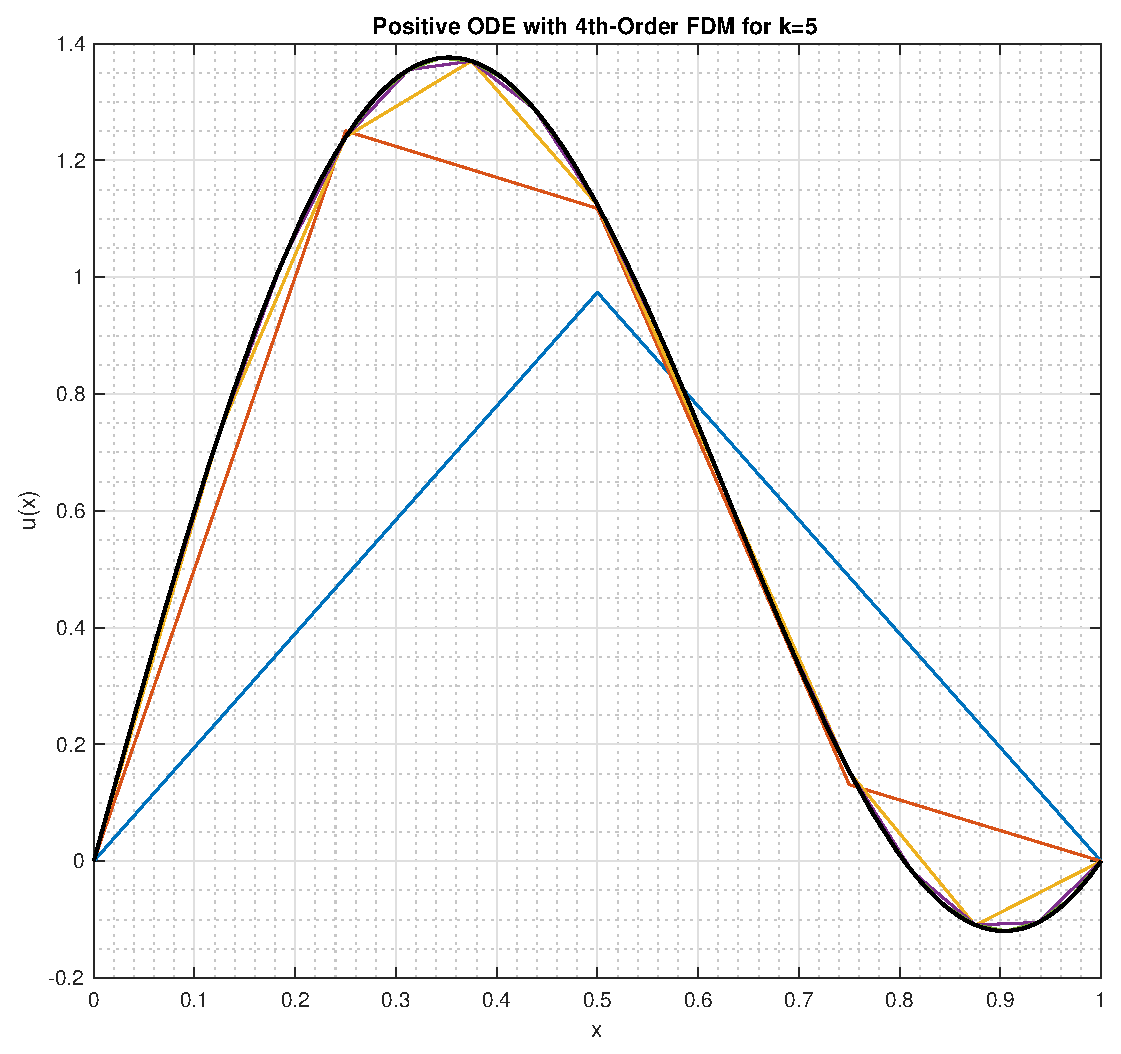
\includegraphics[height = 0.55\linewidth]{positive_ode_order_4_k_5}
%		\caption{Positive ODE -- 4th-Order FDM for $k = 5$}
%	\end{center}
%\end{figure}
%
%\begin{figure}[H]
%	\begin{center}
%		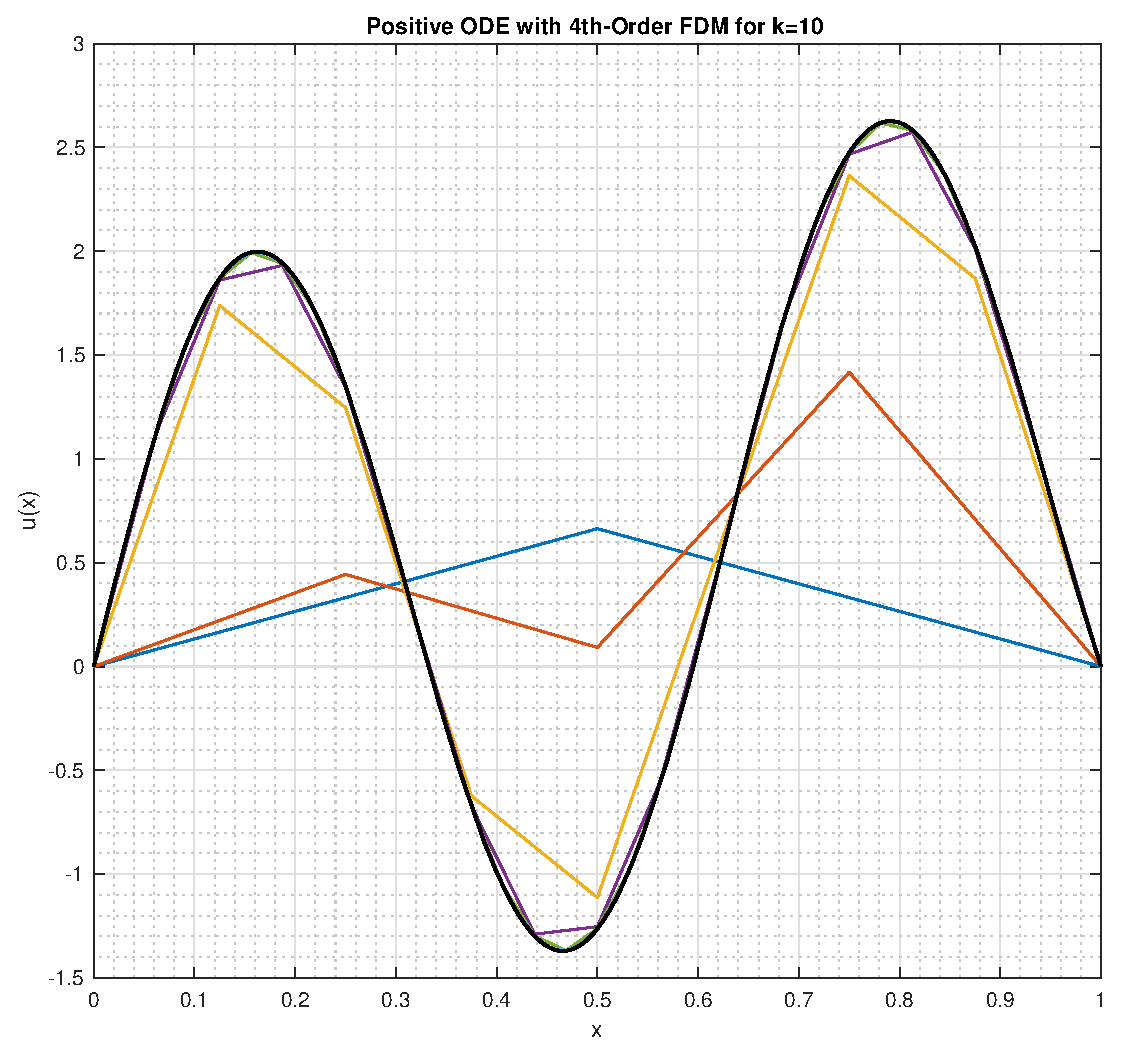
\includegraphics[height = 0.55\linewidth]{positive_ode_order_4_k_10}
%		\caption{Positive ODE -- 4th-Order FDM for $k = 10$}
%	\end{center}
%\end{figure}
%
%\begin{figure}[H]
%	\begin{center}
%		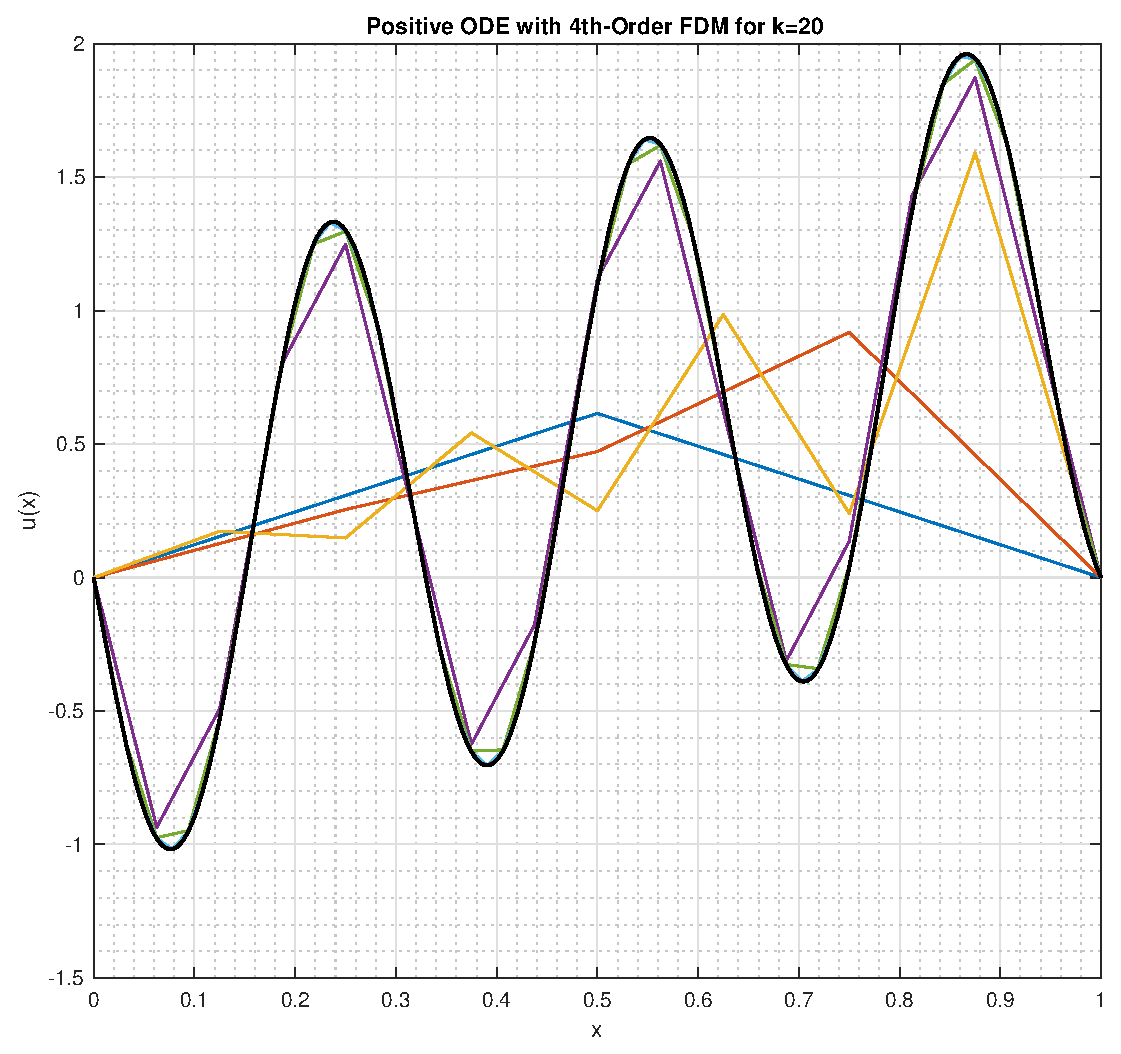
\includegraphics[height = 0.55\linewidth]{positive_ode_order_4_k_20}
%		\caption{Positive ODE -- 4th-Order FDM for $k = 20$}
%	\end{center}
%\end{figure}
%
%\subsubsection{Results -- Negative ODE}
%
%\begin{figure}[H]
%	\begin{center}
%		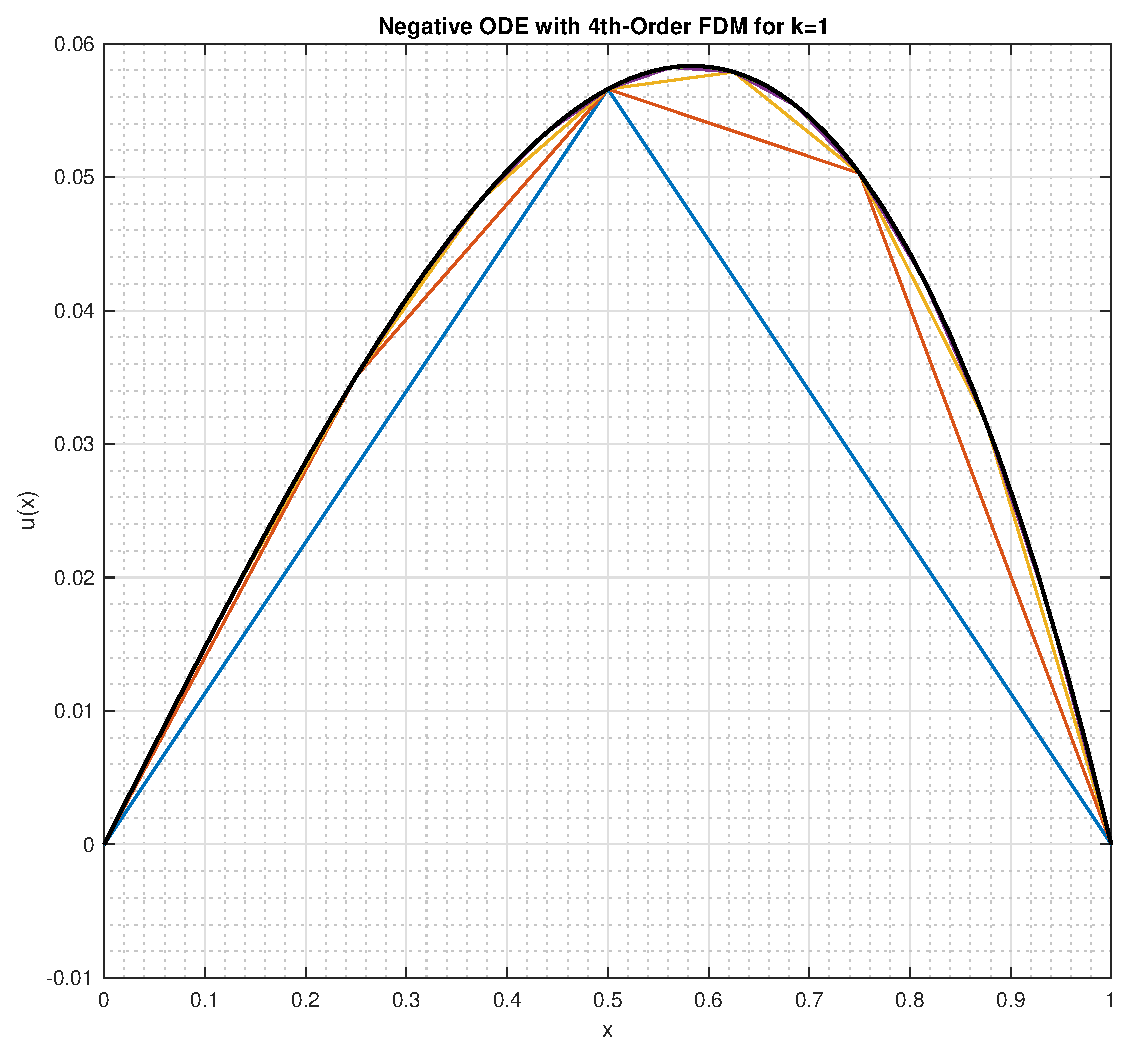
\includegraphics[height = 0.55\linewidth]{negative_ode_order_4_k_1}
%		\caption{Negative ODE -- 4th-Order FDM for $k = 1$}
%	\end{center}
%\end{figure}
%
%\begin{figure}[H]
%	\begin{center}
%		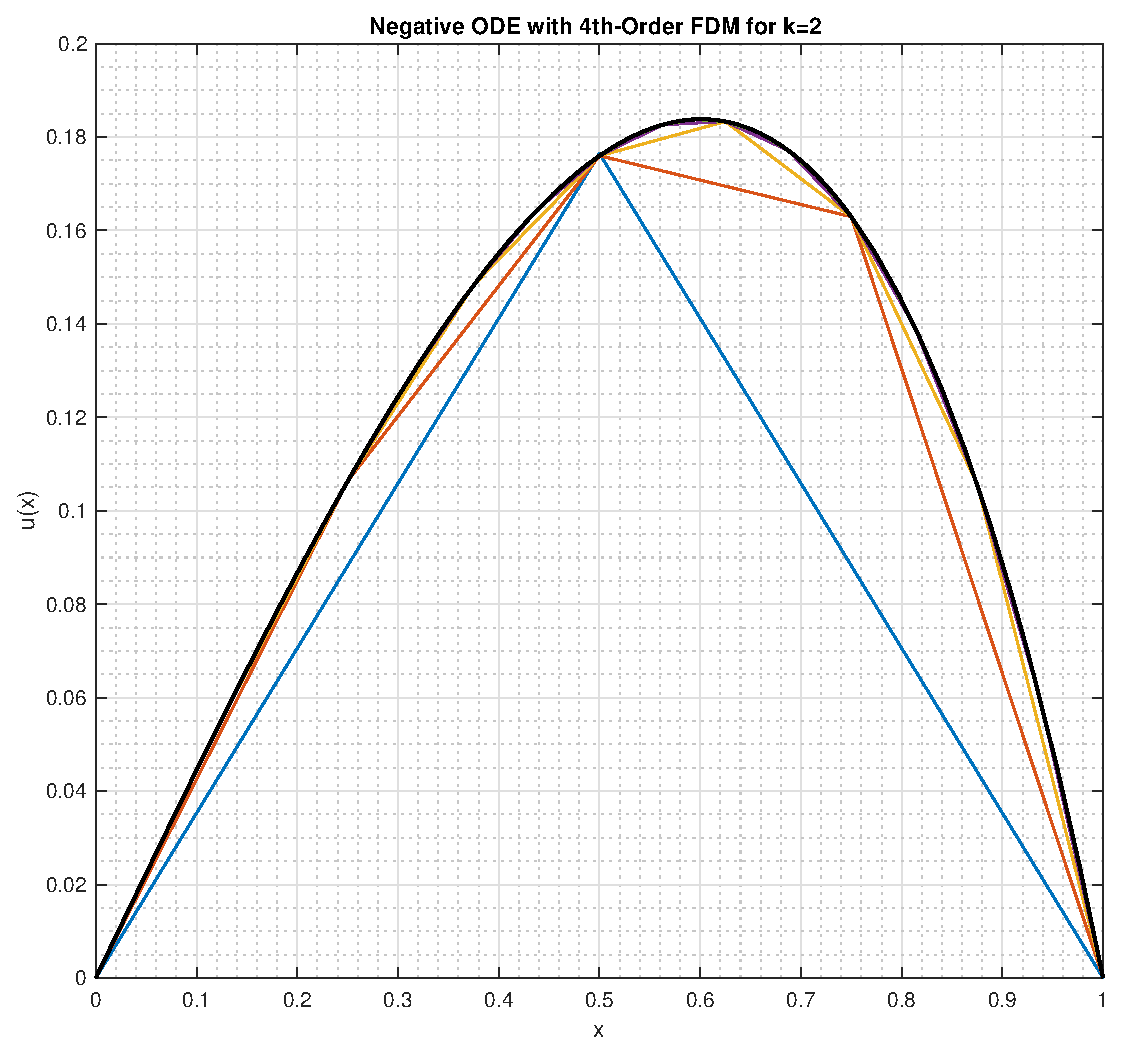
\includegraphics[height = 0.55\linewidth]{negative_ode_order_4_k_2}
%		\caption{Negative ODE -- 4th-Order FDM for $k = 2$}
%	\end{center}
%\end{figure}
%
%\begin{figure}[H]
%	\begin{center}
%		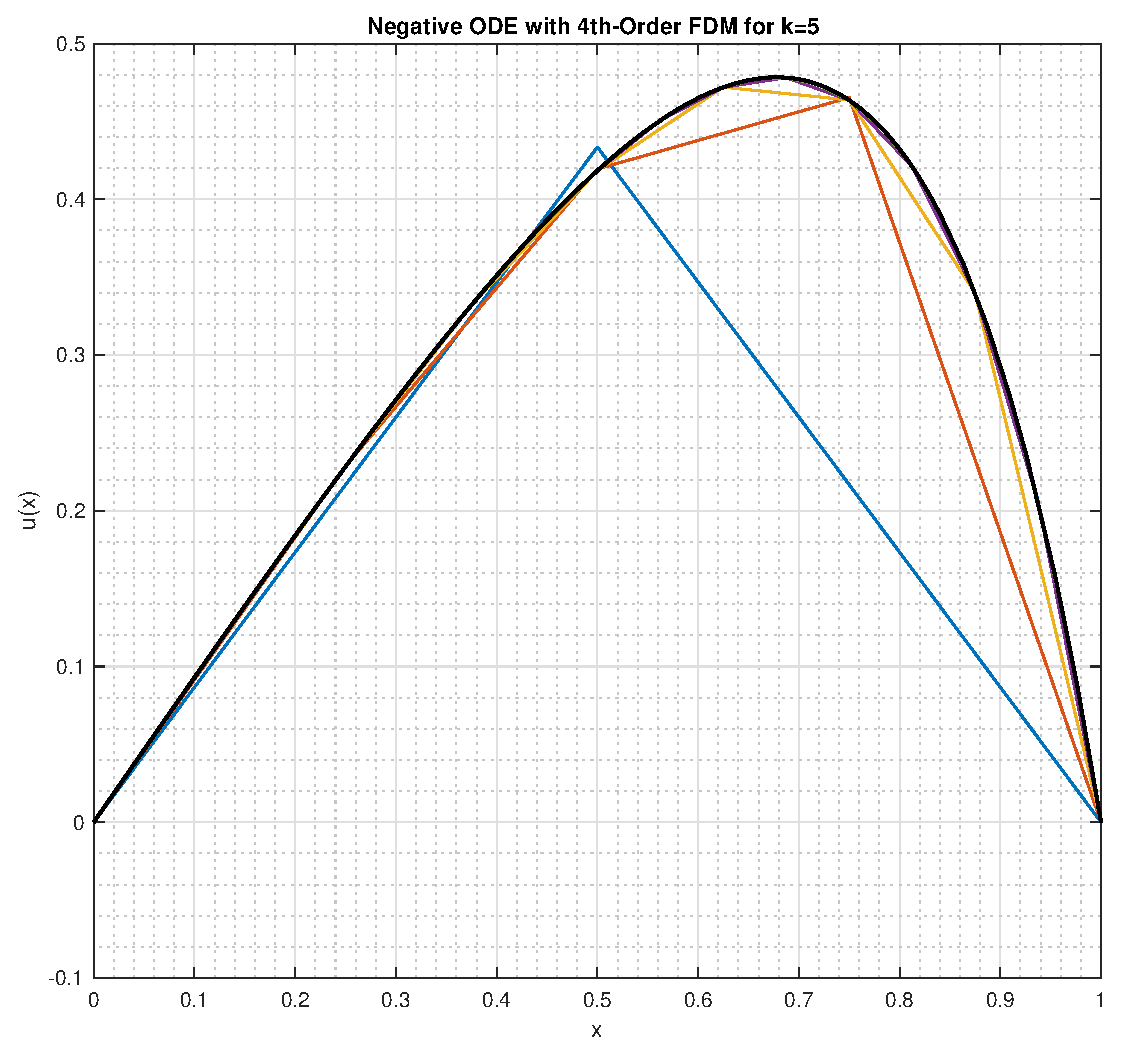
\includegraphics[height = 0.55\linewidth]{negative_ode_order_4_k_5}
%		\caption{Negative ODE -- 4th-Order FDM for $k = 5$}
%	\end{center}
%\end{figure}
%
%\begin{figure}[H]
%	\begin{center}
%		\includegraphics[height = 0.55\linewidth]{negative_ode_order_4_k_10}
%		\caption{Negative ODE -- 4th-Order FDM for $k = 10$}
%	\end{center}
%\end{figure}
%
%\begin{figure}[H]
%	\begin{center}
%		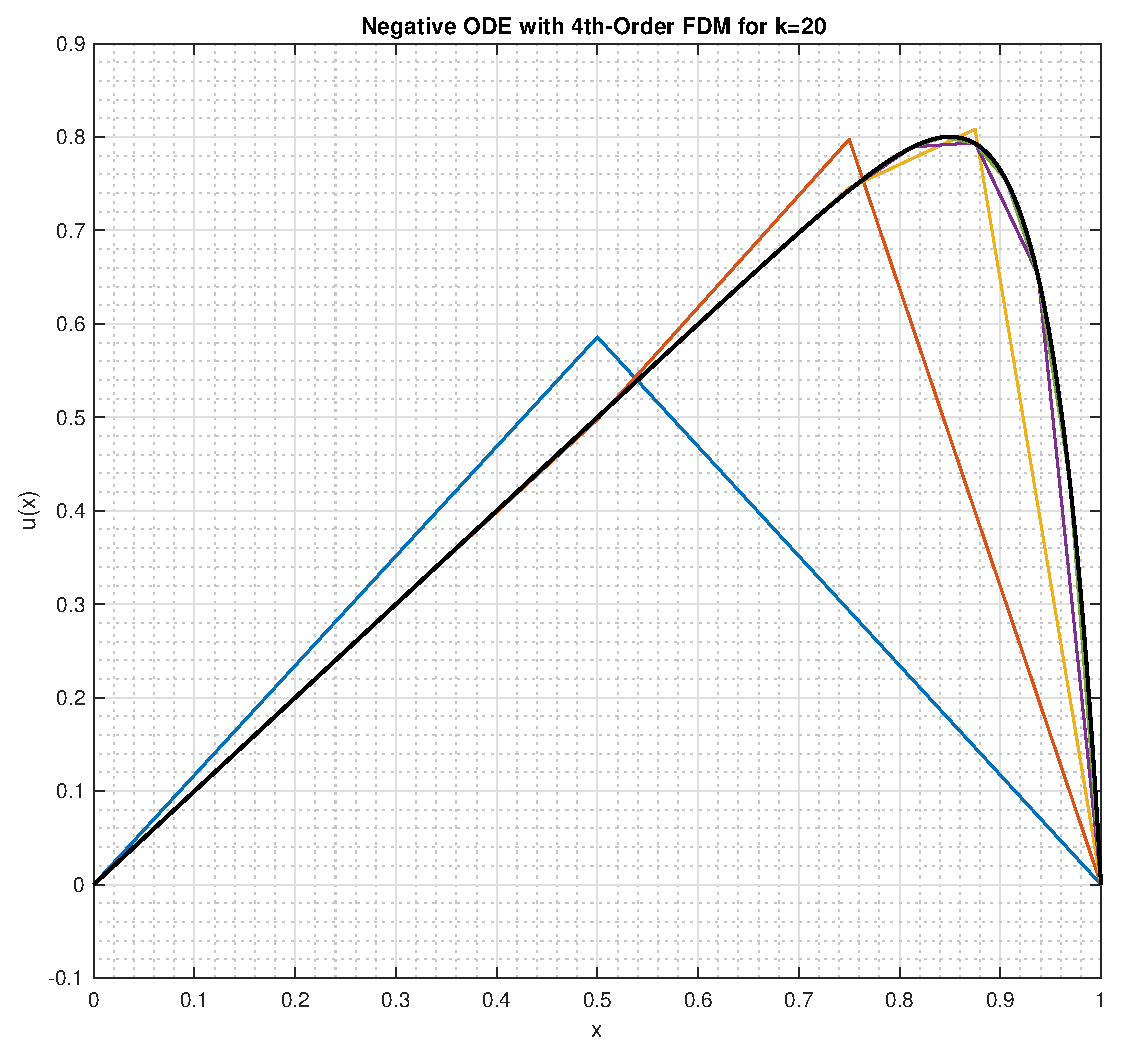
\includegraphics[height = 0.55\linewidth]{negative_ode_order_4_k_20}
%		\caption{Negative ODE -- 4th-Order FDM for $k = 20$}
%	\end{center}
%\end{figure}
%
%\subsubsection{Discussion -- Positive ODE}
%
%\subsubsection{Discussion -- Negative ODE}

\newpage

\section{Convergence Analysis}

\subsection{First-Order First-Derivative Finite Difference Method}

\subsubsection{Derivation}

Developing the Taylor series for $u(x)$ in the vicinity of $x = 1$:
\begin{equation}
u_{N-1} = u_N - \Delta x u'_N + \frac{\Delta x^2}{2} u''_N + \mathcal{O}(\Delta x^3)
\end{equation}
Rearranging terms to solve for $u'_N$:
\begin{equation}
u'_N = \frac{u_N - u_{N-1}}{\Delta x} + \mathcal{O}(\Delta x)
\end{equation}
Switching to a compact notation where $u_N = u_N$, $u_{N-1} = u_{N-1}$, etc.:
\begin{equation}
u'_N = \frac{u_N - u_{N-1}}{\Delta x} + \mathcal{O}(\Delta x)
\end{equation}
Applying the boundary condition $u(1) = u_N = 0$:
\begin{equation}
u'_N = \frac{- u_{N-1}}{\Delta x} + \mathcal{O}(\Delta x)
\end{equation}

From this specific first-derivative formulation at the boundary $x = 1$ using the finite difference method, the approximation can be observed to be first-order ($\mathcal{O}(\Delta x)$).

\subsubsection{Results}

\begin{figure}[H]
	\begin{center}
		\includegraphics[height = 0.55\linewidth]{positive_ode_order_2_fd_order_1}
		\caption{Positive ODE -- 2nd-Order FDM with 1st-Order First-Derivative Approximation}
	\end{center}
\end{figure}

\begin{figure}[H]
	\begin{center}
		\includegraphics[height = 0.55\linewidth]{negative_ode_order_2_fd_order_1}
		\caption{Negative ODE -- 2nd-Order FDM with 1st-Order First-Derivative Approximation}
	\end{center}
\end{figure}

\subsubsection{Discussion}

The positive ODE appears to be less stable than the negative ODE -- a conclusion drawn from the significant deviation from an ideal rate of convergence. This is likely because the solution to the positive ODE can contain numerous oscillations, while the solution to the negative ODE is a single smooth oscillation for every solution. Therefore, the well-behavedness of an ODE solution is a factor in the rate of convergence of a particular finite difference method.

As the above figures indicate, the logarithm of the error decreases roughly at a rate of equal to the negative logarithm of the mesh size. Thus, that the approximation used is first-order accurate and has a rate of convergence of 1.

\subsection{Second-Order First-Derivative Finite Difference Method}

\subsubsection{Derivation}

Developing the Taylor series for $u(x)$ in the vicinity of $x = 1$:
\begin{equation}
u_{N-1} = u_N - \Delta x u'_N + \frac{\Delta x^2}{2} u''_N + \mathcal{O}(\Delta x^3)
\end{equation}
Rearranging terms to solve for $u'_N$, but leaving the second-derivative term:
\begin{equation}
\label{eqn:2o1d}
u'_N = \frac{u_N - u_{N-1}}{\Delta x} + \frac{\Delta x}{2} u''_N + \mathcal{O}(\Delta x^2)
\end{equation}
Returning to the differential equation, rearranging for the second derivative, and evaluating the differential equation at $x = 1$ with corresponding boundary condition $u(1) = u_N = 0$:
\begin{equation}
\pm u''(x)+k^2u(x)=k^2x
\end{equation}
\begin{equation}
u''_N = \pm k^2(1-u_N)
\end{equation}
\begin{equation}
\label{eqn:2o2d}
u''_N = \pm k^2
\end{equation}
This equation yields the exact sign correspondence with the sign of the ODE.

Substituting Equation \ref{eqn:2o2d} into Equation \ref{eqn:2o1d}
\begin{equation}
u'_N = \frac{u_N - u_{N-1}}{\Delta x} \pm \frac{k^2 \Delta x}{2} + \mathcal{O}(\Delta x^2)
\end{equation}
Applying the boundary condition $u(1) = u_N = 0$:
\begin{equation}
u'_N = \frac{-u_{N-1}}{\Delta x} \pm \frac{k^2 \Delta x}{2} + \mathcal{O}(\Delta x^2)
\end{equation}

From this specific first-derivative formulation at the boundary $x = 1$ using the finite difference method, the approximation can be observed to be second-order ($\mathcal{O}(\Delta x^2)$).

\subsubsection{Results}

\begin{figure}[H]
	\begin{center}
		\includegraphics[height = 0.54\linewidth]{positive_ode_order_2_fd_order_2}
		\caption{Positive ODE -- 2nd-Order FDM with 2nd-Order First-Derivative Approximation}
	\end{center}
\end{figure}

\begin{figure}[H]
	\begin{center}
		\includegraphics[height = 0.54\linewidth]{negative_ode_order_2_fd_order_2}
		\caption{Negative ODE -- 2nd-Order FDM with 2nd-Order First-Derivative Approximation}
	\end{center}
\end{figure}

\subsubsection{Discussion}

Like earlier, the positive ODE appears to be less stable than the negative ODE -- a conclusion drawn from the deviation from an ideal rate of convergence. This is likely because the solution to the positive ODE can contain numerous oscillations, while the solution to the negative ODE is a single smooth oscillation for every solution. Therefore, the well-behavedness of an ODE solution is a factor in the rate of convergence of a particular finite difference method.

As the above figures indicate, the logarithm of the error decreases roughly at a rate of 2 times the negative logarithm of the mesh size. Thus, that the approximation used is second-order accurate and has a rate of convergence of 2. It is likely that if a fourth-order finite difference method is used, a fourth-order first-derivative scheme would be needed in order to see the appropriate rate of convergence.

\newpage

\section{MATLAB Code}

\begin{lstlisting}
clear all; close all; clc

%% Initial Conditions

ode.type = 'Positive';
ode.order = 4;

dudx.order = 2;

mesh.order = 1:6;
mesh.dx = 0.5.^mesh.order;

rowID = 0;

%% Boundary Value Problem Solution

for k = [1 2 5 10 20]

	figure
	xlabel('x');    ylabel('u(x)');
	grid on;        grid minor;
	box on;         hold on;
	
	if ode.order == 2
		titleString = strcat(ode.type, ' ODE with 2nd-Order FDM for k=', num2str(k));
	elseif ode.order == 4
		titleString = strcat(ode.type, ' ODE with 4th-Order FDM for k=', num2str(k));
	end
	
	title(titleString)
	
	rowID = rowID + 1;
	colID = 0;
	
	for dx = mesh.dx
	
		nx = 1 / dx + 1;
		x = linspace(0, 1, nx);
		
		A = zeros(nx, nx);
		b = zeros(nx, 1);
		
		if strcmpi(ode.type, 'positive') && ode.order == 2
			alpha = 1 / k^2 / dx^2;
			beta = -2 / k^2 / dx^2 + 1;
		elseif strcmpi(ode.type, 'positive') && ode.order == 4
			alpha = 1 / k^2 / dx^2 + 1/12;
			beta = -2 / k^2 / dx^2 + 10/12;
		elseif strcmpi(ode.type, 'negative') && ode.order == 2
			alpha = -1 / k^2 / dx^2;
			beta = 2 / k^2 / dx^2 + 1;
		elseif strcmpi(ode.type, 'negative') && ode.order == 4
			alpha = -1 / k^2 / dx^2 + 1/12;
			beta = 2 / k^2 / dx^2 + 10/12;
		end
		
		for i = 1:nx
			if i == 1
				A(i, i) = 1;
				b(i) = 0;
			elseif i == nx
				A(i, i) = 1;
				b(i) = 0;
			else
				A(i, i-1) = alpha;
				A(i, i) = beta;
				A(i, i+1) = alpha;
				b(i) = x(i);
			end
		end
		
		u = A\b;
		
		plot(x, u, 'linewidth', 1)
		
		colID = colID + 1;
		
		if strcmpi(ode.type, 'positive') && dudx.order == 1
			dudx.fdm(rowID, colID) = - u(end-1) / dx;
		elseif strcmpi(ode.type, 'positive') && dudx.order == 2
			dudx.fdm(rowID, colID) = - u(end-1) / dx + dx * k^2 / 2;
		elseif strcmpi(ode.type, 'negative') && dudx.order == 1
			dudx.fdm(rowID, colID) = - u(end-1) / dx;
		elseif strcmpi(ode.type, 'negative') && dudx.order == 2
			dudx.fdm(rowID, colID) = - u(end-1) / dx - dx * k^2 / 2;
		end
		
		if strcmpi(ode.type, 'positive')
			dudx.exact(rowID, colID) = 1 - k * cos(k) / sin(k);
		elseif strcmpi(ode.type, 'negative')
			dudx.exact(rowID, colID) = 1 - k * cosh(k) / sinh(k);
		end
	
	end
	
	if strcmpi(ode.type, 'positive')
		fplot(@(x) x-sin(k*x)/sin(k), [0 1], '-k', 'linewidth', 1.5)
	elseif strcmpi(ode.type, 'negative')
		fplot(@(x) x-sinh(k*x)/sinh(k), [0 1], '-k', 'linewidth', 1.5)
	end
	
	legend('\Deltax = (1/2)^1', '\Deltax = (1/2)^2', '\Deltax = (1/2)^3', '\Deltax = (1/2)^4', ...
	'\Deltax = (1/2)^5', '\Deltax = (1/2)^6', 'Analytical Solution', ...
	'location', 'best')
	
	figureString = strcat(lower(ode.type), '_ode_order_', num2str(ode.order), '_k_', num2str(k));
	
	%saveas(gcf, figureString, 'epsc')

end

%% Convergence Analysis

figure
xlabel('-log_{10}(\Deltax)');   ylabel('log_{10}(\epsilon_{rel})');
grid on;                        grid minor;
box on;                         hold on;

logRelError = log10(abs(dudx.exact-dudx.fdm) ./ abs(dudx.exact) * 100);

for kID = 1:5
	plot(-log10(mesh.dx), logRelError(kID, :), '-o', 'linewidth', 1.25);
end

if ode.order == 2 && dudx.order == 1
	titleString = strcat(ode.type, ' ODE with 2nd-Order FDM - 1st-Order First Derivative 
					Approximation');
elseif ode.order == 2 && dudx.order == 2
	titleString = strcat(ode.type, ' ODE with 2nd-Order FDM - 2nd-Order First Derivative 
					Approximation');
elseif ode.order == 4 && dudx.order == 1
	titleString = strcat(ode.type, ' ODE with 4th-Order FDM - 1st-Order First Derivative 
					Approximation');
elseif ode.order == 4 && dudx.order == 2
	titleString = strcat(ode.type, ' ODE with 4th-Order FDM - 2nd-Order First Derivative 
					Approximation');
end

title(titleString)

legend('k=1', 'k=2', 'k=5', 'k=10', 'k=20')

figureString = strcat(lower(ode.type), '_ode_order_', num2str(ode.order), '_fd_order_', 
				num2str(dudx.order));

%saveas(gcf, figureString, 'epsc')
\end{lstlisting}

\end{document}